\documentclass[a4paper,fleqn]{cas-dc}

\usepackage[numbers]{natbib}
% \usepackage[authoryear]{natbib}
% \usepackage[authoryear,longnamesfirst]{natbib}

\usepackage[inline]{enumitem}
\usepackage{hyperref}
\hypersetup{
    % colorlinks = false, % default value = true; used during formatting
    allcolors = {teal}, % color used while writing, recommanded if within guidelines
    % allcolors = {black}, % consistent look
}
\usepackage{cleveref}
\usepackage{placeins}

\newcolumntype{F}{@{\extracolsep{\fill}}>{\global\let\currentrowstyle\relax}l}  % apply row style to column, similar to L
\newcolumntype{H}{@{\extracolsep{\fill}}>{\currentrowstyle}>{\bfseries}c}  % adds bold face to column, similar to C
\newcolumntype{K}{@{\extracolsep{\fill}}>{\currentrowstyle}c}  % forward F style to next columns
\newcolumntype{B}{@{\extracolsep{\fill}}>{\currentrowstyle}>{\color{blue}}c}  % apply blue color to column, similar to C

\newcolumntype{f}{@{\extracolsep{\fill}}>{\global\let\currentrowstyle\relax}>{\color{blue}}l}  % apply row style to column, similar to L
\newcolumntype{o}{@{\extracolsep{\fill}}>{\currentrowstyle}>{\color{blue}}l}  % apply blue color to column, similar to B

\newcommand{\rowstyle}[1]{\gdef\currentrowstyle{#1}#1\ignorespaces}  % apply row style
\newcommand{\bfrow}{\rowstyle{\bfseries}}  % apply bold face to row
\newcommand{\bluerow}{\rowstyle{\color{blue}}}  % apply blue color to row
\newcommand{\responsemod}{\color{blue}}
\newcommand{\responsemodsm}[1]{\textcolor{blue}{#1}}
\newcommand{\captionb}[1]{\caption{\responsemodsm{#1}}}
\newcommand{\sectionb}[1]{\section{\responsemodsm{#1}}}
\newcommand{\subsectionb}[1]{\subsection{\responsemodsm{#1}}}
\newcommand{\subsubsectionb}[1]{\subsubsection{\responsemodsm{#1}}}

\def\tsc#1{\csdef{#1}{\textsc{\lowercase{#1}}\xspace}}
\tsc{WGM}
\tsc{QE}


\renewcommand{\dblfloatpagefraction}{0.1}

\begin{document}
\let\WriteBookmarks\relax
\def\floatpagepagefraction{1}
\def\textpagefraction{.001}

\shorttitle{Novel approach to identify suitable machine learning model  in the healthcare industry}

\shortauthors{Ketkar Y., Gawade S.}

\title [mode = title]{A Decision Support System for Selecting the Most Suitable Machine Learning in Healthcare using User Parameters and Requirements.}

\let\printorcid\relax

\author[1]{Yashodhan Ketkar}
\ead{ketkaryapr19me@student.mes.ac.in}
\affiliation[1]{organization={Department of Information Technology Engineering, Pillai College of Engineering},
    % addressline={}, 
    city={New Panvel},
    % citysep={}, % Uncomment if no comma needed between city and postcode
    postcode={410206},
    % state={Maharashtra},
    country={India}}

\author[2]{Sushopti Gawade}
\ead{sgawade@mes.ac.in}
\affiliation[2]{organization={Department of Computer Engineering, Pillai College of Engineering},
    % addressline={}, 
    city={New Panvel},
    %          citysep={}, % Uncomment if no comma needed between city and postcode
    postcode={410206},
    % state={Maharashtra},
    country={India}}

\begin{abstract}
    The use of machine learning in various fields is still limited. The driving reason behind this is the lack of easy-to-use systems for non-technical people. The objective of this paper is to provide the general population access to a machine learning system. We propose an automated machine learning system for non-technical users. The proposed system automates the selection of the best model as per user requirements. The proposed methods employ both the performance of the model and user requirements in the form of preferences for the model selection. The combination of these two features is calculated as the Vscores of the models. In this study, we employed the proposed system on Parkinson's disease datasets. The Support Vector Machine (SVM) and Random Forest (RF) are used as the algorithms for training the two models in the system. The system selected SVM as the best suited model for three test cases and the RF Model as the best suited model for one case. The proposed system showed high base accuracy in training the machine learning models and in the selection of appropriate models. Performed tests showed that the time parameter significantly affected the Vscore of the model.
\end{abstract}

% Use if graphical abstract is present
%\begin{graphicalabstract}
%\includegraphics{}
%\end{graphicalabstract}

% Research highlights
% \begin{highlights}
% \item a
% \item a
% \item a
% \end{highlights}

% Keywords
% Each keyword is seperated by \sep
\begin{keywords}
    Automated Selection System \sep
    General Prediction System \sep
    Healthcare Industry \sep
    Parkinson's Disease Detection \sep
    Supervised Learning Algorithms
\end{keywords}

% \tolerance 9999
% \hbadness=10000

\maketitle


% Main text

\section{Introduction}\label{sec:introduciton}

In recent years, machine learning has become very popular. Earlier, machine learning was limited to the research field. But quite recently, it has been used in various fields [\citenum{ref_paper_36}]. This is partially due to the increasing availability of computers and to the growth in computing power.

Researchers are using machine learning in various fields. One such field is solar energy production. In this field, the prediction of solar radiation available per day can be very significant. \cite*{ref_paper_7} employed a few machine learning algorithms for the prediction of the amount of solar radiation received in a day. \citeauthor{ref_paper_7} used natural properties such as weather, time, etc. as features for the machine learning algorithms. \citeauthor{ref_paper_7} concluded that supervised learning models gave satisfactory results in predicting the amount of solar radiation. \citeauthor{ref_paper_7} concluded that the Artificial Neural Network (ANN) model showed great potential for such specialized tasks.

In the field of chemistry, there is a wide range of factors that need to be considered. \cite*{ref_paper_10} used machine learning in the field of chemistry. \citeauthor{ref_paper_10} suggest that the models performed better than conventional statistical methods. \citeauthor{ref_paper_10} concluded that more research is necessary before implementation.

Machine learning can be applied to network security for intrusion detection. \cite*{ref_paper_21} state that the supervised learning methods perform satisfactorily for intrusion detection. \citeauthor{ref_paper_21} also remark that the supervised learning methods are limited to conventional problems.

\cite*{ref_paper_24} notes a lack of information and meaningful research in the medical field. \citeauthor{ref_paper_24} suggests that more support, subject-specific scope, and accuracy are important factors for the higher impact of machine learning in the medical field. \citeauthor{ref_paper_24} also suggests that the ideal system should be able to take multiple data types for training.

\cite*{ref_paper_29} used machine learning with a combination of Internet of Things (IoT) for smart cities. \citeauthor{ref_paper_29} conclude that machine learning shows promising results for smart cities. \citeauthor{ref_paper_29} remark that machine learning is able to handle the high volume of data generated by sensors. \cite*{ref_paper_12} suggests that machine learning can handle downstream tasks efficiently.

This suggests that even with the immense popularity and accessibility of machine learning, it is still underutilized by the general population. This can be attributed to a lack of knowledge and skills. To solve this problem, we are proposing a system with minimum user interaction. The proposed system can be operated by users without prior knowledge of machine learning. This system allows them to train their machine learning algorithms.

The proposed system can be deployed on a local network. The system can feed data either manually or automatically according to user needs and policies. The local deployment also limits external access and reduces the influence of external factors on data.

\sectionb{Literature review}\label{sec:literature_review}

{\responsemod
    Supervised machine learning algorithms are widely used in various fields. The study conducted on the application of machine learning in various industries suggests that machine learning is already being utilized in various industries \cite{ref_paper_14}. Supervised machine learning shows excellent results for well-labeled datasets. Such as in the case of Civil Structural Health Monitoring (SHM) machine learning, where supervised machine learning algorithms showed satisfactory results \cite{ref_paper_6}.
    
    Supervised learning algorithms are very efficient for conventional problems. The machine learning systems are capable of detecting Distributed Denial of Service (DDOS) attacks very accurately. The DDOS attack is a conventional network attack with various known features. Hence, the supervised algorithms are very successful in the prevention of such attacks in real time \cite{ref_paper_9}.
    
    The study was conducted on the automated selection of support vector machine (SVM) algorithms with the goal of selecting the most optimal SVM model for the given tasks \cite{ref_paper_2}. It was noted that the hyperparameters and the used data have an extreme impact on the prediction time of the algorithm.
    
    Recently, machine learning was used in the diagnosis of Coronavirus Disease 2019 (COVID-19) disease and studies related to its structure. The survey of various studies was taken with various types of dataset \cite{ref_paper_20}. These studies suggested that the supervised learning algorithms showed promising results in the diagnosis of COVID-19.
    
    Machine learning is widely used in the diagnosis process, such as in the diagnosis of Parkinson's disease. In this study, a machine learning system used for the detection of Parkinson's disease achieved up to 100\% accuracy with a confidence level higher than 95\%. The study used Random Foreset (RF) and SVM algorithms \cite{ref_paper_34}. The inclusion of machine learning in diagnosis leads to better results and higher accuracy while working with the high volume of data \cite{ref_paper_15}. From a survey of over 200 published studies, it was noted that the machine learning system with supervised algorithms improved clinical decisions in Parkinson's disease diagnosis \cite{ref_paper_27}. The study was conducted on the use of various machine learning models and resulted in SVM outperforming other models \cite{ref_paper_30}.
    
    Arrhythmia is an irregular heartbeat, which is a common symptom of cardiological disorders. The supervised learning methods have already been used for the detection of arrhythmias with high accuracy and sensitivity \cite{ref_paper_16}. Good feature selection and selection guidelines result in better performing machine learning systems \cite{ref_paper_28}. With the help of the SVM model \cite{ref_paper_38}, 91.2\% accuracy is obtained in the detection of arrhythmia.
    
    The machine learning system needs to be robust, extremely accurate, and easy to use. The system that fulfills these essential requirements and provides early detection of arrhythmia is critical for better treatment of patients \cite{ref_paper_4}.
    
    The Long Short Term Memory (LSTM), SVM, and Multiplayer Perceptron (MLP) models were used on the ECG signals of COVID-19 patients. These models were used with robots to successfully monitor the patient's data and condition. The SVM model produced satisfactory results \cite{ref_paper_40}.
    
    The study of the automated selection of machine learning algorithms and their hyperparameters showed the limitations of the biomedical industry \cite{ref_paper_32}. One of these limitations is the security and privacy aspects of the machine learning solution. While machine learning systems have great potential in healthcare systems, more research is needed to handle the security and privacy aspects \cite{ref_paper_37}.
    
    A machine learning system that complies with Health Insurance Portability and Accountability Act (HIPPA) regulations was able to achieve up to 83\% accuracy in the detection of heart disease \cite{ref_paper_41}. A machine learning system with a multiperceptron neural network achieved up to 78\% accuracy for stroke prediction with a relatively small dataset. The system was capable of producing even better results with large training datasets \cite{ref_paper_42}.
    
    Machine learning utilizes various approaches to the same problem. In a study, two approaches were used to solve a diagnostic problem. In a direct approach, data is fed to a machine learning model. In an indirect approach, data is equalized before the machine learning process. The indirect method showed better results compared to the direct method. While the experiment was successful, it was noted that machine learning is still unstable for the medical field \cite{ref_paper_8}.
    
    The supervised learning methods are extremely effective in the medical field and have proved useful in reducing the number of errors caused by humans \cite{ref_paper_11}. The survey about the use of machine learning in the medical field suggested that big companies are already using the machine learning system for various tasks such as diagnosis and research. This introduced the need for a machine learning system that could be available to non-technical people. These systems should be able to handle various types of data \cite{ref_paper_33}.
    
    There is a sufficient amount of literature available about automated machine learning systems. The automated system performed better than standalone systems, as observed from various benchmarks \cite{ref_paper_a_5}. The use of an automated system reduces the complexity of the problems compared to regular machine learning systems \cite{ref_paper_a_1}. The ability to handle high throughput of the data is another benefit of the automated system \cite{ref_paper_a_3}. The automated systems are used as graph learning systems, with various frameworks already available in the industry \cite{ref_paper_a_4}. The preprocessing pipelines in the automation system are able to handle large amounts of data as the results of tests improve with each iteration \cite{ref_paper_a_12}.
    
    The automated system will allow non-technical people to use machine learning. The optimal SVM kernal selection with automated optimal hyperparameter calculations was performed with minimal hunman interaction. The system was able to calculate up to 2 hyperparameters with no human interaction \cite{ref_paper_3}. Two other studies also focused on the selection of the optimal hyperparameters. In one of these studies, neural networks were used, while in the other study, a genetic algorithm was applied \cite{ref_paper_a_14,ref_paper_39}. Use of genetic algorithms was able to reduce uncertainty in the predictions of the system \cite{ref_paper_39}.
    
    The automatic selection process can be extremely beneficial in dynamic environments. The excavation of soil or tunneling is one such environment. The displacement induced by excavation was predicted by machine learning with properties of soli as features. The unsupervised machine learning algorithm Genetic Algorithm Multilayer Perceptron (GA-MLP) showed good potential, while automated machine learning was found to be the most optimal algorithm in these dynamic conditions \cite{ref_paper_1}. It is noted that machine learning systems are extremely successful in dynamic environments \cite{ref_paper_1,ref_paper_13}. An automated machine learning system, used to enhance the academic performance of students, produced up to 75.9\% accuracy. The system used data prior to the start of the academic year to predict the performance of the students. The system is able to detect the probability of failure with 83\% accuracy \cite{ref_paper_a_7}.

    There are multiple ways to select the best-suited model. The important part of such a system is the selection system. The system uses various approaches for selection; ranking is one of those approaches. The meta ranking is an alternative to the baseline ranking system. This system uses a multi-criteria ranking system for the selection of ideal classifiers \cite{ref_paper_23}.
    
    Automated machine learning systems are already used in the medical field. Automated machine learning is employed for clinical note analysis \cite{ref_paper_a_2} and the detection of breast cancer \cite{ref_paper_a_6} by gene analysis. An automated system of twenty machine learning algorithms with graphical and web based interfaces for protein sequences has been deployed in one of the studies \cite{ref_paper_a_11}. Recently, during the COVID-19 pandemic, an automated machine learning system was used for the purpose of screening. 98.3\% accuracy was achieved during the screening \cite{ref_paper_a_15}. The triage system and the survival rate prediction system were built with an automated machine learning system during the COVID-19 pandemic \cite{ref_paper_a_9}.
    
    The civil engineering field also employed machine learning systems. An automated system was used during the disaster planning by studying the complex dynamics of glabal landslides \cite{ref_paper_a_10}. Another automated system, which was deployed to automate the workflow, performed consistently and objectively \cite{ref_paper_a_13}. An automated machine learning system was used to observe the physical and hydraulic soils for an accurate measurement of the soil moisture content. This system was able to extract the features from the data without human interaction \cite{ref_paper_a_8}.
}

\sectionb{Design and implmentation}\label{sec:design_and_implmentation}

\subsectionb{Mathematical model}\label{subsec:mathematical_model}

The system is able to work with multiple models. So let's assume we have N number of models, Model 1, Model 2,$\cdots$, Model N for the task. Each model has six performance parameters, they are Accuracy P$_1$, F1 Score P$_2$, Precision P$_3$, Recall P$_4$, Area under ROC (Receiver Operating Characteristic) P$_5$ and Prediction Time P$_6$. Each parameter is assigned a predefined weight depending on the user's requirements. These performance parameters and weights are used to evaluate the total performance score of models. The performance score of the model is obtained by subtracting the weighted time parameter from the summation of weighted parameters.

\begin{equation}\label{eq:V_score_formula}
    V_{score} = \left(\sum_{x=1}^5 w_xP_x\right) - w_6P_6
\end{equation}

The Vscore of each model is calculated with \cref{eq:V_score_formula}. For a given N number of models, we will get V$_1$, V$_2$, $\cdots$, V$_n$. The model with the highest Vscore will be selected as the best-suited model.

\subsubsectionb{Weightage}\label{subsubsec:weightage}

The weights in the system are selected by the user's requirements. The weights are calculated by the system. The value of weight lies within the range of 0.2 and 1. The default weights for the first five parameters are set to 0.6. The weights of parameters are dependent on each other, except for the sixth (time) parameter, which is independent of other parameters. In the case of the sixth parameter, the default weight is set at 0.5. The value can be changed to either 0.25 or 0.75 with respect to the user's requirements.

\subsectionb{System architecture}\label{subsec:system_architecture}

{\responsemod
    The goal of the system is to be used by non-technical users. \Cref{fig:model_process} shows the mathematical model and system architecture in detail. As shown in the figure, part of the user requirements are used for the generation of models. This information contains the model templates along with predermined hyperparameters for model generation. With this template, the models are generated and trained with 80\% of the training dataset. The remaining 20\% of the dataset is used for the testing process for the extraction of performance parameters. As mentioned earlier, six parameters are used in this system. These parameters are forwarded to the Vscore calculation process. In this process, the user requirements are used to generate the weightage for each parameter. These weighted parameters are used to calculate the Vscore mentioned earlier. In the next step, these Vscores are compared, and the model with the higher Vscore is selected as the most suited model. The selected model is stored in the system for future use along with the performance parameters of the model.
}

\begin{figure*}[ht]
    \centering
    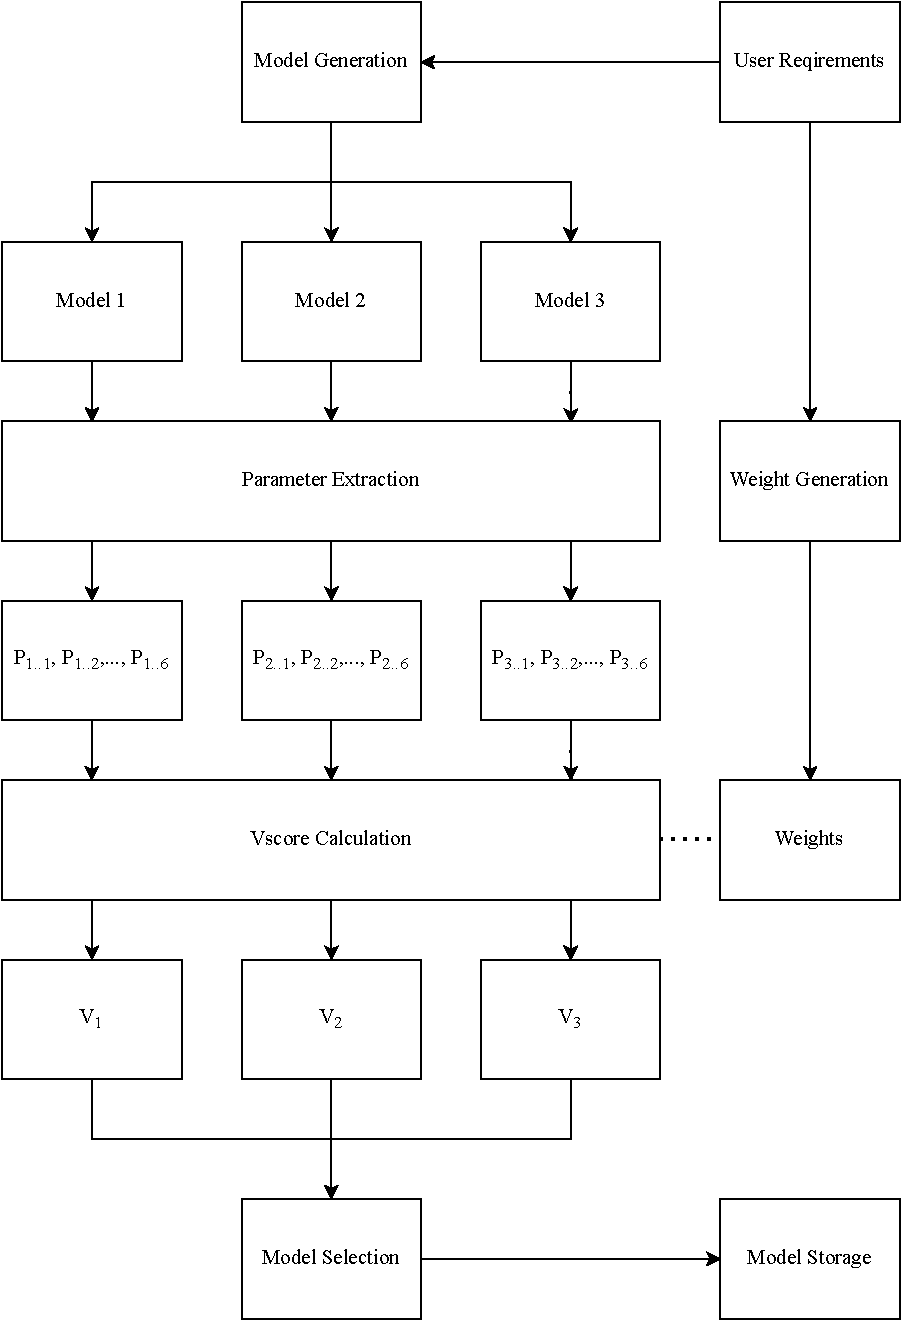
\includegraphics[width=1.6\columnwidth]{math_model_relaxed_flow.pdf}
    \caption{Model Process}
    \label{fig:model_process}
\end{figure*}

\subsectionb{System processes}\label{subsec:system_processes}

{\responsemod
    The system consists of three processes, or modules. These processes are the training process, selection process, and prediction process. The first two processes interact with each other. Their task is to produce the best-suited model for the user's needs. The third process interacts with the selected models to generate the predictions. The user is indirectly allowed to access the training and prediction process. The user data is stored on a local drive for easier and faster access. The following subsection will give a further explanation of these processes.
}

\subsubsectionb{Training process}\label{subsubsec:training_process}

The training process is the first process in the system. \Cref{fig:training_process} shows the structure of the training process. The training process has many functions. The first function is gathering data from the user and preprocessing it for training purposes. The training process also generates models with the template, which contains model structure and parameters. These models are trained with processed data and stored for future use. The performance of models is also calculated during this phase and stored for selection purposes.

\begin{figure}[ht]
    \centering
    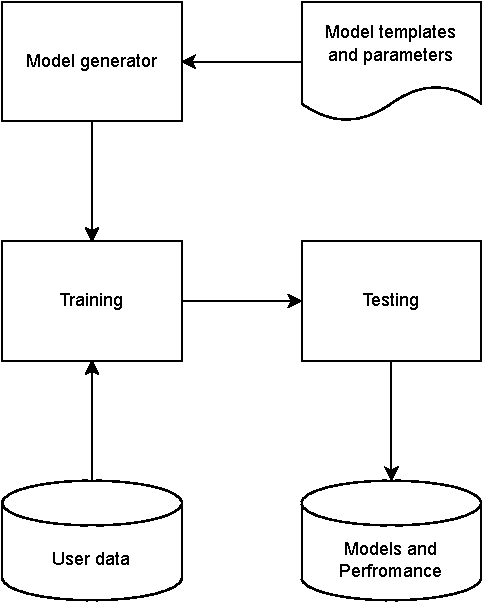
\includegraphics[width=0.7\columnwidth]{training_and_testing.pdf}
    \caption{Training Process}
    \label{fig:training_process}
\end{figure}

\subsubsectionb{Selection process}\label{subsubsec:selection_process}

The selection process is second in the system. \Cref{fig:selection_process} shows the structure of the training process. This process evaluates the performance of models based on metrics and weightage. The metrics of models are generated during the training process. The performance weightage is defined by the user depending on requirements. The final performance score is calculated and used for the selection of the best model for user's task. The selected model is stored in a separate directory with a label for easier access. This model will be used for prediction problems.

\begin{figure}[ht]
    \centering
    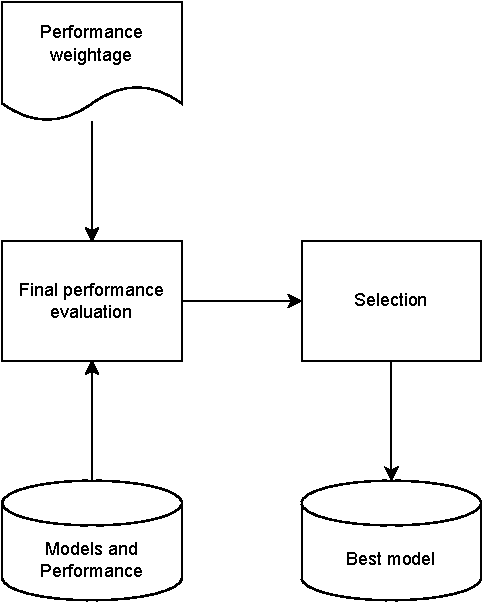
\includegraphics[width=0.7\columnwidth]{selection.pdf}
    \caption{Selection Process}
    \label{fig:selection_process}
\end{figure}

\subsubsectionb{Prediction process}\label{subsubsec:prediction_process}

The prediction process is the final process in the system. \Cref{fig:prediction_process} shows the structure of the prediction process. This process unpacks the best model and loads it for prediction. The model generates predictions with user-provided data. The output is displayed to the user. This output is also stored for future reference.

\begin{figure}[ht]
    \centering
    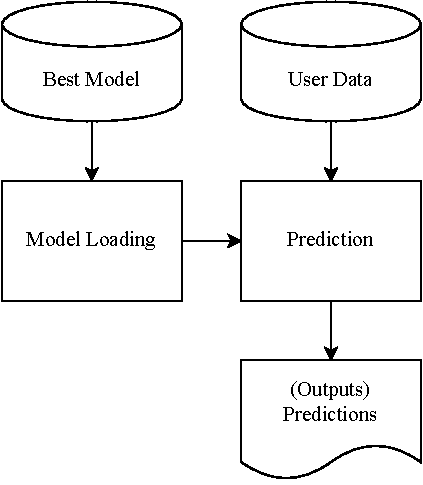
\includegraphics[width=0.7\columnwidth]{prediction.pdf}
    \caption{Prediction Process}
    \label{fig:prediction_process}
\end{figure}

\subsection{Algorithms}\label{subsec:algorithms}

The system uses two algorithms to run. These algorithms are training and selection algorithms and prediction algorithms.

\vspace{-0.5em}

\subsubsectionb{Training and selection algorithm}\label{subsubsec:training_and_selection_algorithm}
\vspace{0.5em}
\begin{enumerate}
    \item Collect and receive dataset.
    \item Split data into an 80:20 ratio for training and testing.
    \item Build a model from presets.
    \item Train models with training datasets and store models.
    \item Evaluate the performance of models with the testing dataset.
    \item Rank models with the help of performance and premade tuning parameters.
    \item Select the best model and store it for future use.
\end{enumerate}

\vspace{-0.5em}

\subsubsectionb{Prediction algorithm}\label{subsubsec:prediction_algorithm}
\vspace{0.5em}
\begin{enumerate}
    \item Collect and receive dataset.
    \item Then load the best-suited model data from the storage.
    \item Unpack the model for predictions.
    \item Make predictions with the provided dataset and loaded model.
    \item Return predictions to the user.
\end{enumerate}

\subsection{Implmentation}\label{subsec:implmentation}

\subsubsectionb{Web architecture}\label{subsubsec:web_architecture}

The system provides service with a web application. The users aren't allowed to interact with the system directly. This provision is to provide security and reduce the outside influence on results. The interface layer is used for a user to interact with the system indirectly. \Cref{fig:web_architecture} shows the web architecture of the system. The system is connected to the database directly. A direct connection is provided to access live data. The user is provided with a list of uploaded (user uploaded) datasets along with the preference options. The user selects a training dataset from this list and provides preference according to its needs. A user-selected dataset is processed by the system and stored in the database. The user provided preferences are used for the weightage generation. Currently, the system only allows staff members to access the results and patient data, and training options are restricted to people with admin roles.

\begin{figure}[ht]
    \centering
    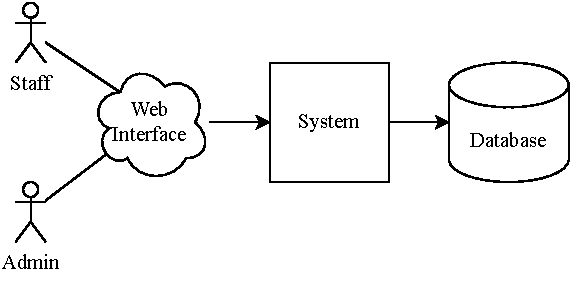
\includegraphics[width=0.9\columnwidth]{web_architecture.pdf}
    \caption{Web Architecture}
    \label{fig:web_architecture}
\end{figure}

\subsubsectionb{Web interface}\label{subsubsec:web_interface}

The web interface provides users with a way to interact with the system. The primary function of the web interface is to provide secure access to the system process. Approved users can interact with various modules on the system. This interface allows users to access selection and prediction processes. Users can upload data to the system.

The interface presents prediction results as well as performance evaluation results. Prediction results are provided in tabular format and stored in Comma Separated Values (CSV) files for future reference. Performance results are presented in graphical format and also stored in CSV files for future reference.

\sectionb{Result and analysis}\label{sec:result_and_analysis}

\subsectionb{Dataset and test cases}\label{subsec:dataset_and_test_cases}

To test the selection system we are employing two models and one dataset. The dataset contains 201 records with 754 features [\citenum{parkinsons_disease_detection}]. The random forest algorithm and support vector machine algorithm is used to generate the models Model$_1$ and Model$_2$ respectively. The performance obtained from these two models is shown in \cref{tab:performance_analysis_of_dataset}. The table shows the base performance of two models. This base performance will be weighted to calculate the Vscore of the models.

\begin{table}[ht]
    \caption{Performance Analysis of Dataset}\label{tab:performance_analysis_of_dataset}
    \begin{tabular*}{\tblwidth}{@{}LLLL@{}}
        \toprule
        Performance Parameter & Model$_1$ & Model$_2$ \\
        \midrule
        $P_1$ \quad Accuracy & 0.8039 & 0.7451 \\
        $P_2$ \quad F1 Score & 0.8750 & 0.8434 \\
        $P_3$ \quad Pricision & 0.8537 & 0.7955 \\
        $P_4$ \quad Recall & 0.8974 & 0.8974 \\
        $P_5$ \quad Area under ROC & 0.6987 & 0.5737 \\
        $P_6$ \quad Prediction Time & 0.5563 & 0.0981 \\
        \bottomrule
    \end{tabular*}
\end{table}

We will use 4 cases to test the system. The test cases are:

\noindent
{\bfseries Case I:} We did not provide any preference in the selection parameters. Hence the default weight for all parameters. The default weightage of the system is 0.6 for the first five parameters and 0.5 for the time parameter.

\vspace*{0.5em}
\noindent
{\bfseries Case II:} We gave preference to parameters in this order:
\begin{enumerate*}[label=\arabic{*}.]
    \item Accuracy (1.0)
    \item Pricision (0.8)
    \item Area under ROC (0.6)
    \item F1 Score (0.4)
    \item Recall (0.2).
\end{enumerate*}

\noindent
Also, the sixth parameter (prediction time) is set to careful approach (0.25).

\vspace*{0.5em}
\noindent
{\bfseries Case III:} In this case, we used similar preferences from previous case except for the sixth parameter, where we selected default approach (0.50).

\vspace*{0.5em}
\noindent
{\bfseries Case IV:} Similar to the previous case we only changed the sixth parameter to the faster approach (0.75).

\vspace*{0.5em}
\Cref{tab:wieghtage_for_cases}, shows the weight values for each case. These values are calculated with the help of the priority set by users. These values range between 0.2 and 1.0, and the sum of the first five weights is equal to 3.0.

\begin{table}[h]
    \caption{Weightage for cases}\label{tab:wieghtage_for_cases}
    \begin{tabular*}{\tblwidth}{@{}LLLLL@{}}
        \toprule
        Weights & Case$_1$ & Case$_2$ & Case$_3$ & Case$_4$ \\
        \midrule
        $w_1$ & 0.6 & 1.0 & 1.0 & 1.0 \\
        $w_2$ & 0.6 & 0.4 & 0.4 & 0.4 \\
        $w_3$ & 0.6 & 0.8 & 0.8 & 0.8 \\
        $w_4$ & 0.6 & 0.2 & 0.2 & 0.2 \\
        $w_5$ & 0.6 & 0.6 & 0.6 & 0.6 \\
        $w_6$ & 0.50 & 0.25 & 0.50 & 0.75 \\
        \bottomrule
    \end{tabular*}
\end{table}

\subsectionb{Test results}\label{subsec:results_and_discussion}
We used \cref{eq:V_score_formula} to calculate the Vscore of the models. \Cref{tab:results_of_test_cases}, shows the Vscore of Model$_1$ and Model$_2$ values along with the model selected by the system.

As seen in \cref{tab:results_of_test_cases}, Model$_2$ is selected as the best model in three out of four cases. While Model$_1$ is selected as the best model is Case II, where we gave preference to a careful approach. The time parameter played an important role in the selection of the models compared to the other five parameters. Hence, implementation of the time parameter proved beneficial in the final selection of the model. \Cref{fig:vscore_of_test_cases} shows this result (Vscores) in graphical format.

\begin{table}[ht]
    \caption{Results of test cases}\label{tab:results_of_test_cases}
    \begin{tabular*}{\tblwidth}{@{}LCCL@{}}
        \toprule
        Case & $V_{score}|$Model$_1$ & $V_{score}|$Model$_2$ & Model Selected \\
        \midrule
        I & 2.19907 & 2.26402 & Model$_2$ \\
        II & 2.29648 & 2.21802 & Model$_1$ \\
        III & 2.15741 & 2.19351 & Model$_2$ \\
        IV & 2.01834 & 2.16899 & Model$_2$ \\
        \bottomrule
    \end{tabular*}
\end{table}

\begin{figure*}[ht]
    \centering
    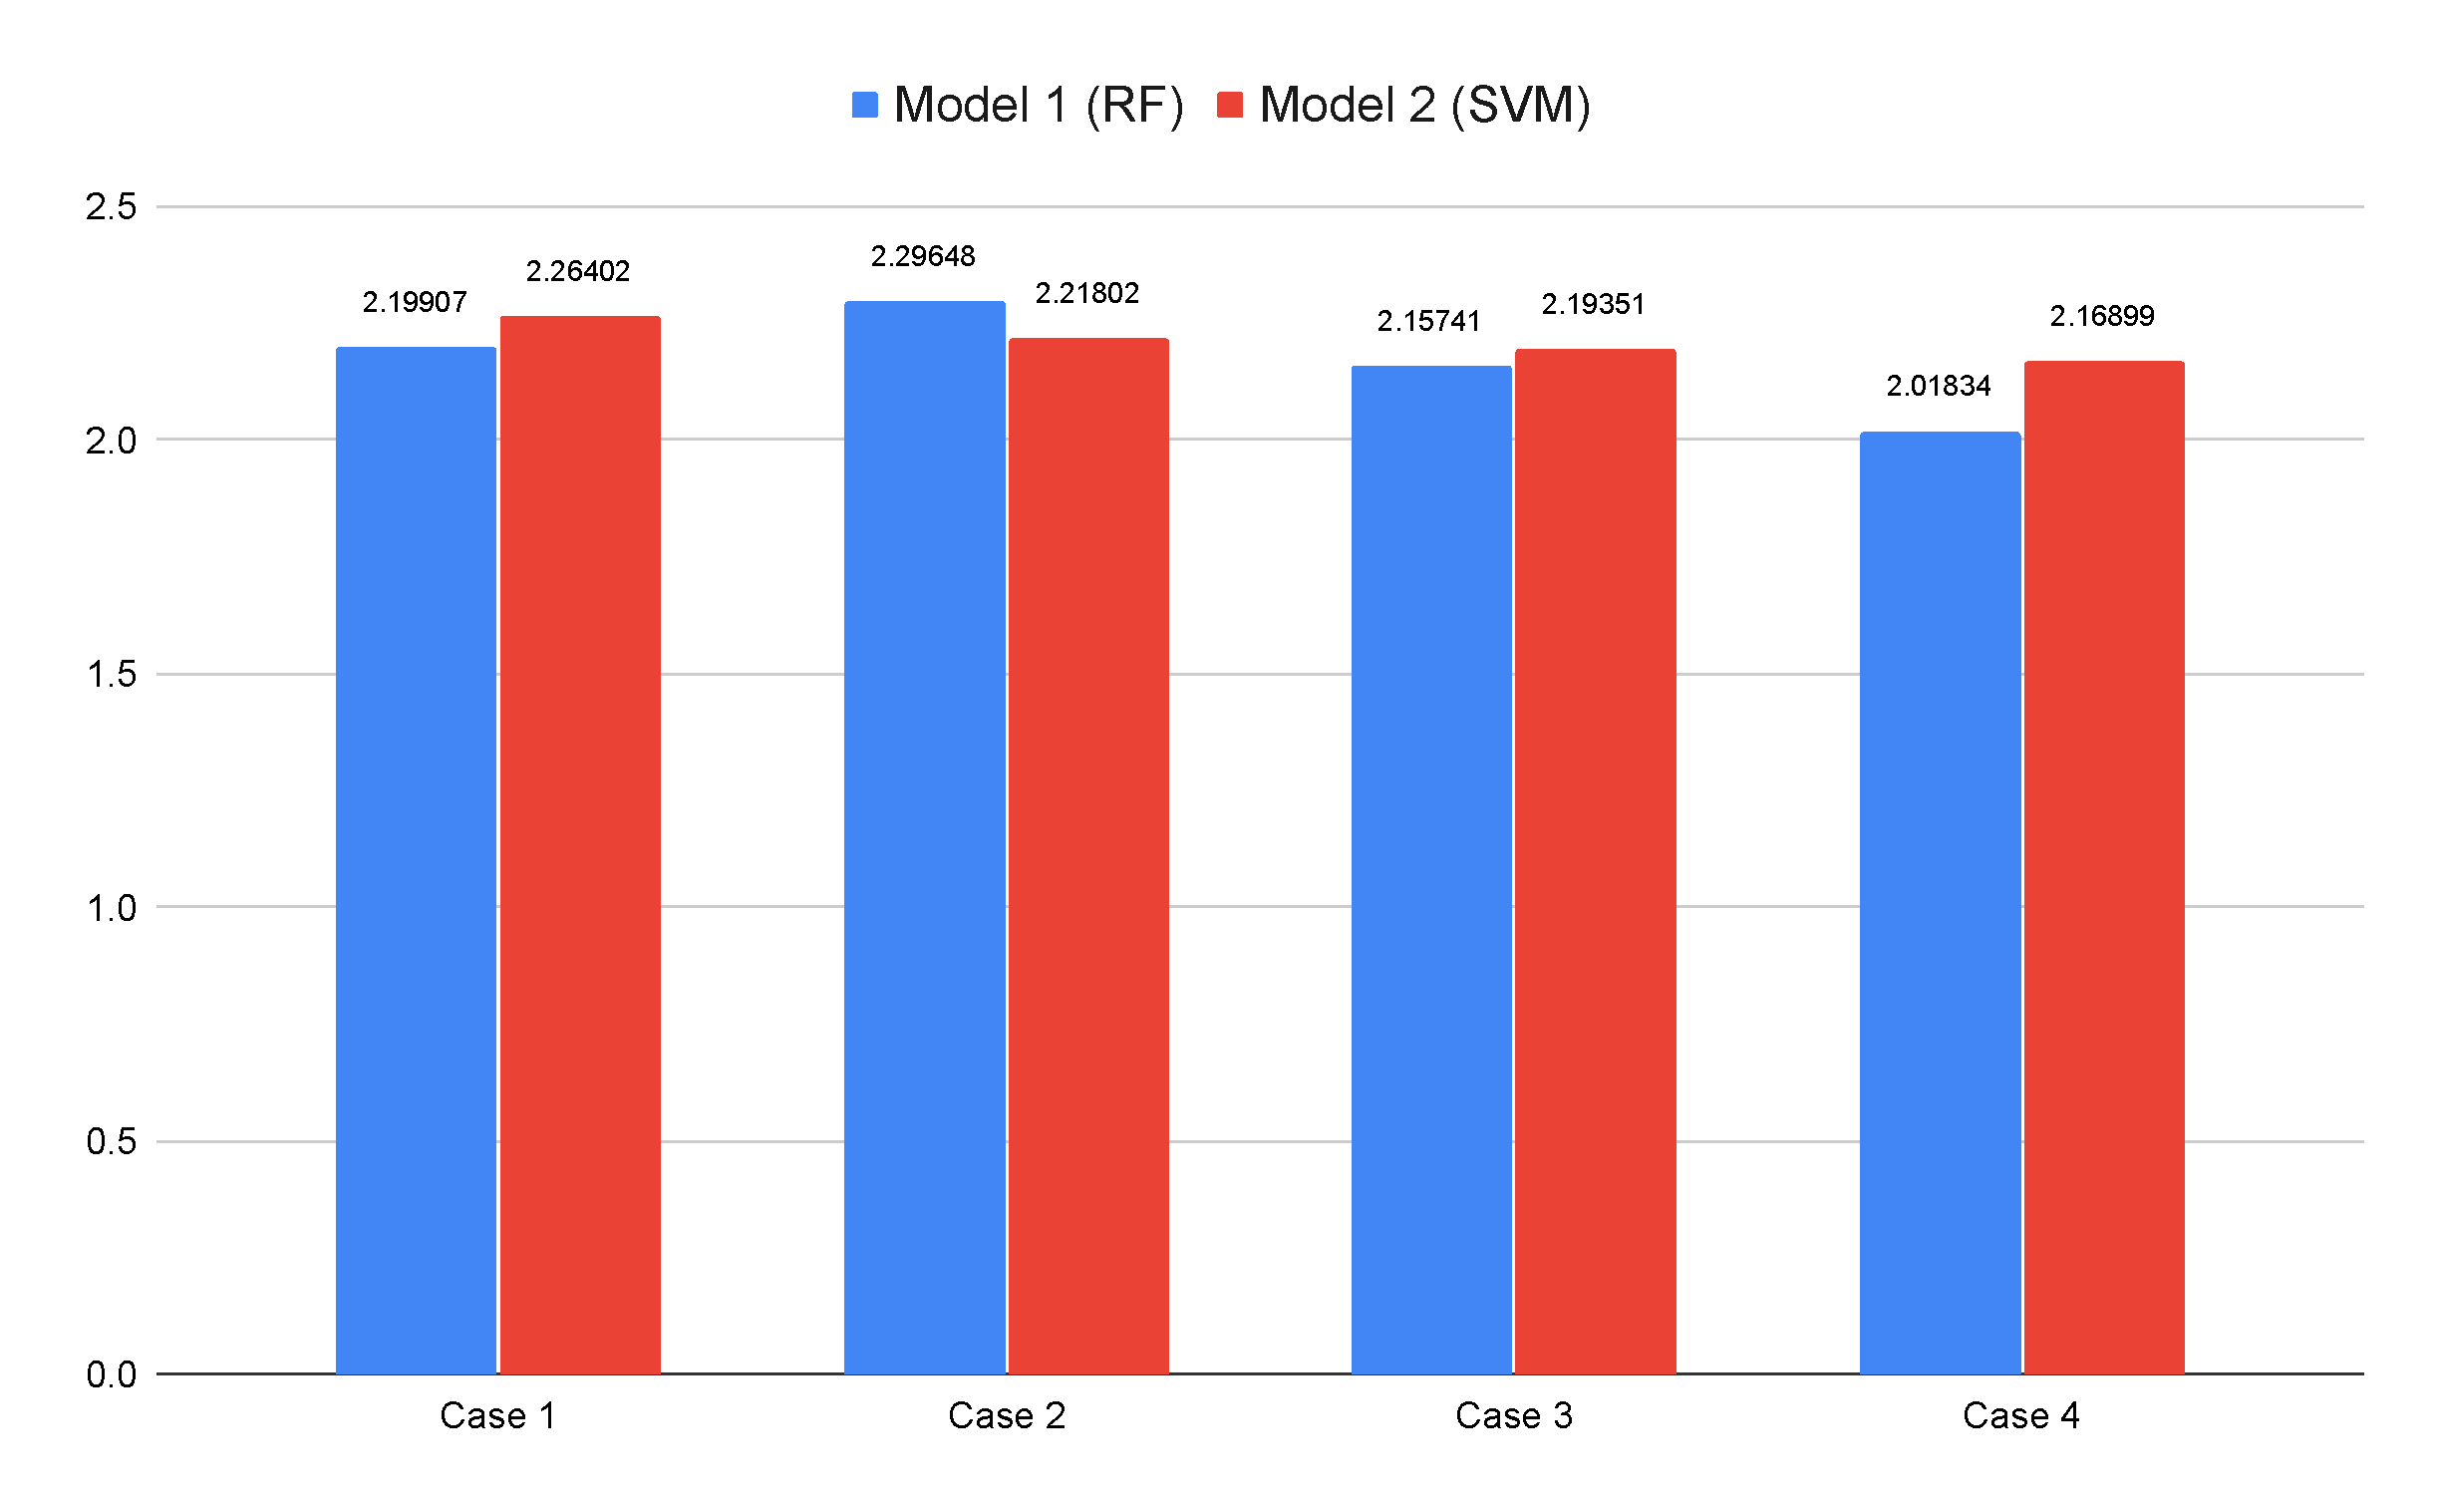
\includegraphics[width=2\columnwidth]{result_test_cases.pdf}
    \caption{Vscore of test cases}
    \label{fig:vscore_of_test_cases}
\end{figure*}

\subsubsectionb{Key findings}\label{subsubsec:key_findings}

From the data displayed in previous section, we saw how the system works on different datasets. These are a few key findings we obtained from that knowledge.
\setlist{nosep}
\begin{enumerate}
    \item The system successfully works with two different models.
    \item The scale of data does impact the efficiency and effectiveness of the system.
    \item The system successfully uses the weightage generated from the user requirements.
    \item The weightage of the user, especially the weight for time parameter significantly impacts the decision of the system.
\end{enumerate}

{\responsemod
\section{Novelty of the work}\label{sec:novelty_of_the_work}

The suggested system in this paper is a weightage based model selection system. The novelty of the system is the combination of the user selected preferences and the performance parameters of the models for the selection of the most suited model. The system is able to handle a large number of models, which are generated by the templates provided by the user. The suggested system can work automatically with minimal human interaction. The user is only required to provide the training data to the system. The system will use this data to select the most suitable model. The user can use options to select preferred parameters, otherwise default values will be used in the selection process.
}

\sectionb{Conclusion and future work}\label{sec:conclusion_and_futur_work}

The system performed satisfactorily during the tests. The application was able to select the model for the provided dataset. The best-suited model was able to meet the user requirements. The whole process required minimum human interaction. The system can be used with any number of models. It allows users with limited prior knowledge easier access to machine learning technology. The user-defined parameter weights lead to the selection of the best-suited model for particular tasks. The performance of models is stored for future evaluation of the system.

Currently, the system is limited to only supervised machine learning algorithms. The supervised nature of these algorithms limits the training dataset to the labeled dataset. By providing support to unsupervised learning algorithms, systems can accommodate various types of training datasets. The selection parameters are adjusted before the training process. These predefined parameters restrict the selection choices of the system. Allowing users to tweak selection parameters after the training process will allow them to meet user requirements more efficiently. Future work will also focus on the implementation of Robotic Process Automation (RPA) tools for the data collection for easier integration with the old system [\citenum{ref_paper_self_rpa}]. Future work will also focus on comparing the performance between the proposed system and similar automation systems.


% \FloatBarrier
% \newpage


% Numbered list
% Use the style of numbering in square brackets.
% If nothing is used, default style will be taken.
%\begin{enumerate}[a)]
%\item 
%\item 
%\item 
%\end{enumerate}  

% Unnumbered list
%\begin{itemize}
%\item 
%\item 
%\item 
%\end{itemize}  

% Description list
%\begin{description}
%\item[]
%\item[] 
%\item[] 
%\end{description}  

% Figure
% \begin{figure}[<options>]
% 	\centering
% 		\includegraphics[<options>]{}
% 	  \caption{}\label{fig1}
% \end{figure}


% \begin{table}[<options>]
% \caption{}\label{tbl1}
% \begin{tabular*}{\tblwidth}{@{}LL@{}}
% \toprule
%   &  \\ % Table header row
% \midrule
%  & \\
%  & \\
%  & \\
%  & \\
% \bottomrule
% \end{tabular*}
% \end{table}

% Uncomment and use as the case may be
%\begin{theorem} 
%\end{theorem}

% Uncomment and use as the case may be
%\begin{lemma} 
%\end{lemma}

%% The Appendices part is started with the command \appendix;
%% appendix sections are then done as normal sections
%% \appendix

% \section{}\label{}

% To print the credit authorship contribution details
\printcredits

%% Loading bibliography style file
%\bibliographystyle{model1-num-names}
\raggedright
\bibliographystyle{cas-model2-names}

% Loading bibliography database
\bibliography{cas-refs.bib}

% Biography
\bio{}
% Here goes the biography details.
\endbio

% \bio{pic1}
% Here goes the biography details.
\endbio

\end{document}

